% ==============================================================================
%
%                                    DVG303
%                  Objektorienterad design och programmering
%                                Laboration #1
%
% Author:   Jonas Sjöberg
%           Högskolan i Gävle
%           tel12jsg@student.hig.se
%           https://github.com/jonasjberg
%
% License:  Creative Commons Attribution-NonCommercial-ShareAlike 4.0
%           International.  See LICENSE.md for full licensing information.
% ==============================================================================

\renewcommand{\thesubsection}{(\alph{subsection})}

\section{Uppgift 3}\label{sec:uppg3}

\subsection{}\label{sec:uppg3a}
\subsubsection*{Frågeställning}
Betrakta nu modellen en gång till: Ser ni likheter när det gäller objektens
beteenden? Vilka är dessa? Ge en Beskrivning!

\subsubsection*{Lösning}
Alla figurer behöver någon mekanism för att flytta på sig och det kan tänkas
att alla figurer skulle kunna använda sig av sammma logik för att utföra
förflyttningen. Exempel på hur det skulle kunna implementeras är med en
\texttt{move()}-metod i en gemensam superklass som itererar genom en lista av
\texttt{Vertex2D}-punkter och flyttar varje punkt för sig. Alla figurer kan
uttryckas med en lista av punkter och kan således ärva från en gemensam
superklass.
\par Ett annat exempel är rotering, som inte är applicerbart för vissa figurer,
t.ex. cirkeln. Det kan vara konceptuellt möjligt att rotera en perfekt cirkel,
men i det här fallet så skulle cirkelns interna läge inte förändras, och
den grafiska representationen skulle inte heller komma att ändras.
Alternativet till ett interface \texttt{Rotatable} i fallet med cirkeln är att
\texttt{rotate()}-metoden i cirkel-klassen blir ersatt med en tom metod genom 
\emph{override}.


\subsection{}\label{sec:uppg3b}
\subsubsection*{Frågeställning}
Utöka nu klassdiagrammet en gång till: Lägg till minst ett interface som
deklarerar någon metod som passar till det som ni beskrev ovan. Låt klasserna
implementera interfacet ifall det passar!

\subsubsection*{Lösning}
Jag bestämde mig för att lägga till interfacen \texttt{Movable},
\texttt{Rotatable} och \texttt{Scalable}. Detta med motiveringen att det
är operationer som efterfrågas i användningsfallsdiagrammet och som de olika
figurerna kan komma att behöva utföra på olika vis, beroende på figur. 
Avvägning gjordes mot att göra en enklare design som förlitar sig mer på arv
och \emph{override} av superklassers metoder. Det uppdaterade klassdiagrammet
återfinns i Figur~\ref{fig:uppg3b}.

%\begin{figure}[htbp]
\begin{sidewaysfigure}[ht]
\centering
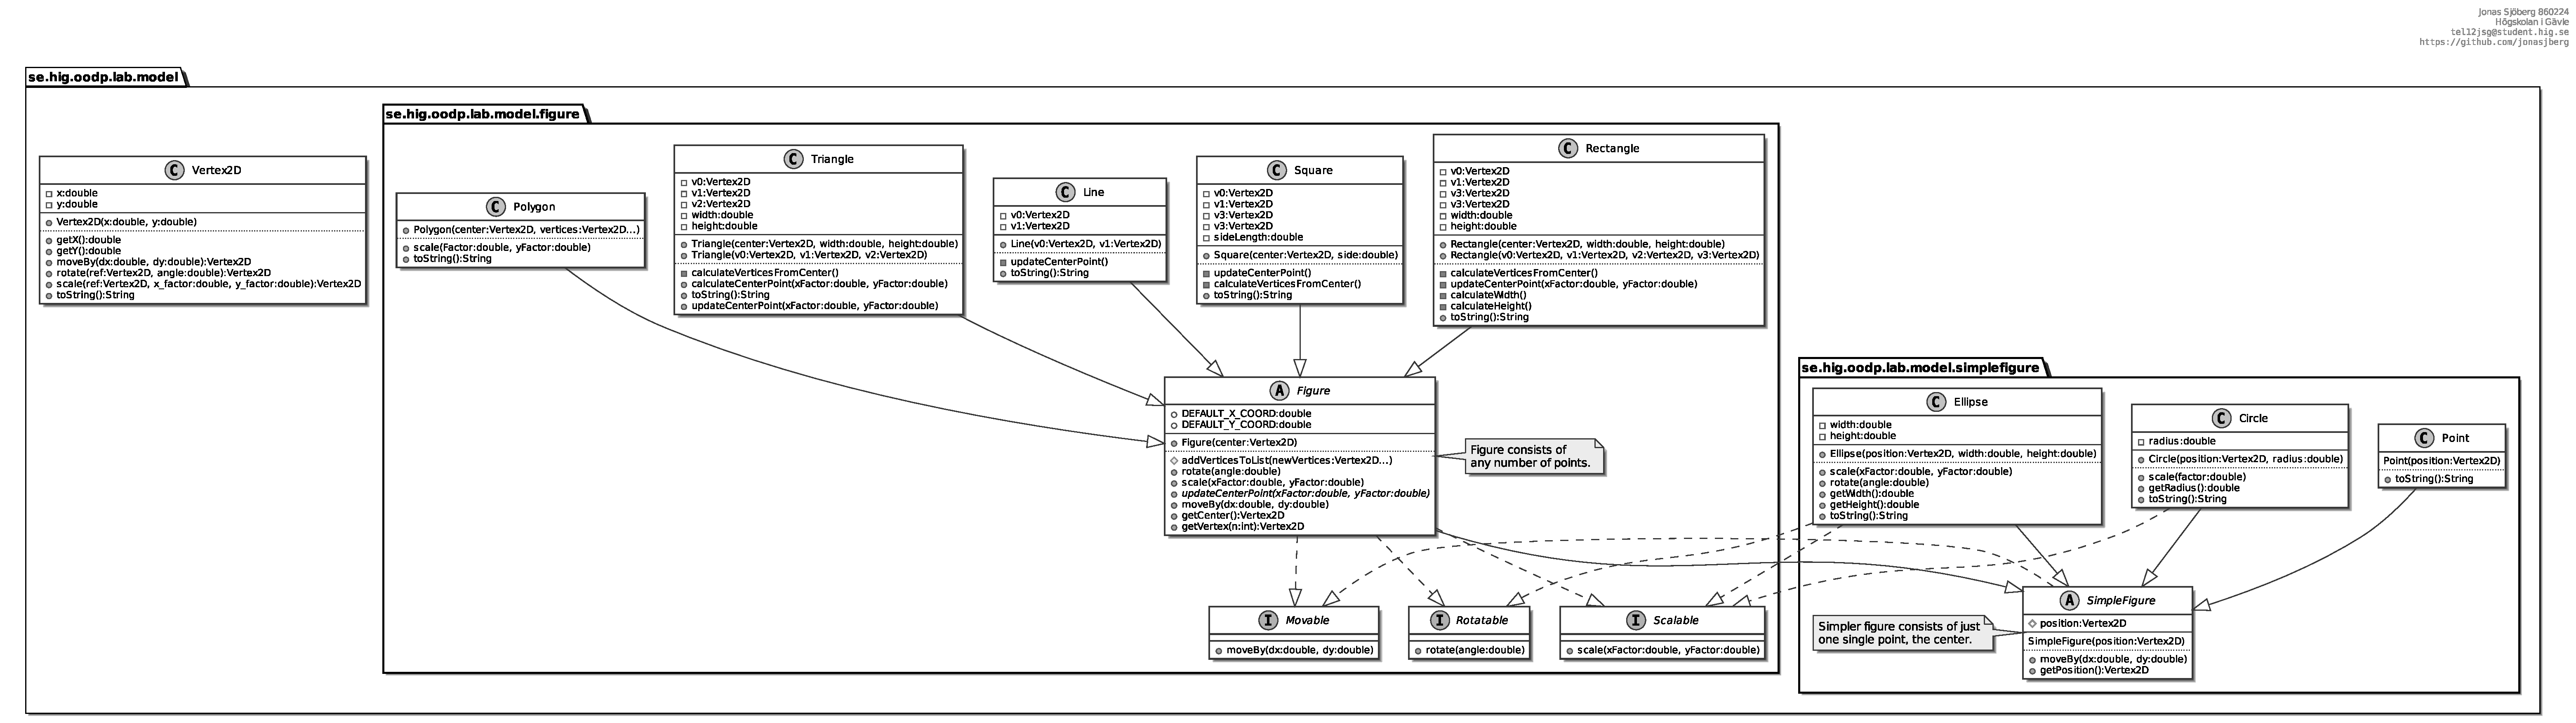
\includegraphics[width=\linewidth]{diagram/uppgift3.eps}
\caption{Uppgift~3\ref{sec:uppg2c}: UML-diagram för geometriska figurer
(\texttt{diagram/uppgift3.eps})}
\label{fig:uppg3b}
\end{sidewaysfigure}



\subsection{}\label{sec:uppg3c}
\subsubsection*{Frågeställning}
Uppdatera koden från uppgift 2 så att det motsvarar den utökade modellen från
(b)!

\subsubsection*{Lösning}
Se bifogad kod för implementering.


